\documentclass[caret-main.tex]{subfiles}
\begin{document}
\subsection*{Binary Classification}
\subsubsection*{Defining true/false positives}
In general, Positive = identified and negative = rejected. Therefore:

\begin{itemize}
\item True positive = correctly identified

\item False positive = incorrectly identified

\item True negative = correctly rejected

\item False negative = incorrectly rejected
\end{itemize}
\subsubsection*{Medical testing example:}
\begin{itemize}
\item True positive = Sick people correctly diagnosed as sick

\item False positive= Healthy people incorrectly identified as sick

\item True negative = Healthy people correctly identified as healthy

\item False negative = Sick people incorrectly identified as healthy.
\end{itemize}
%-------------------------------------------------- %
\newpage
\subsection*{Steps in building a prediction}
\begin{enumerate}
\item Find the right data
\item Define your error rate
\item Split data into:
\begin{itemize}
\item Training Set
\item Testing Set
\item Validation Set(optional)
\end{itemize}
\item On the training set pick features
\item On the training set pick prediction function
\item On the training set cross-validate

\item If no validation - apply 1x to test set
\item If validation - apply to test set and refine
\item If validation - apply 1x to validation
\end{enumerate}
%-------------------------------------------------------%
\subsection*{Question 1}
Which of the following (pick one) is \textbf{NOT} a step in building a prediction model?
\subsubsection*{Options}
\begin{itemize}
\item[(i)] Defining the error rate			
\item[(ii)] Picking features			
\item[(iii)] Obtaining the right data			
%\item Selecting features with the test set.
\item[(iv)] Estimating test set accuracy with training-set accuracy. 
\item[(v)] (N0) Selecting features with the test set.
\end{itemize} 
\newpage
\subsection*{Cross Validation}
Bias Variance Trade-off \textit{http://scott.fortmann-roe.com/docs/BiasVariance.html}
\begin{itemize}
\item In a prediction problem, a model is usually given a dataset of known data 
on which training is run (\textit{training dataset}), and a dataset of unknown data (or \textit{first seen data/ testing dataset}) against which testing the model is performed.
\item Cross-validation is mainly used in settings where the goal is prediction, and one wants to estimate how accurately a predictive model will perform in practice. 
\item The goal of cross validation is to define a dataset to "test" the model in the training phase (i.e., the validation dataset), in order to limit problems like overfitting, give an insight on how the model will generalize to an independent data set (i.e., an unknown dataset, for instance from a real problem), etc.
\item Cross-validation is important in guarding against testing hypotheses suggested by the data (called "Type III errors"), especially where further samples 
are hazardous, costly or impossible to collect 
\end{itemize}
\subsubsection*{K-fold cross validation}
\begin{itemize}
\item In k-fold cross-validation, the original data set is randomly partitioned into $k$ equal size subsamples. 
\item Of the $k$ subsamples, a single subsample is retained as the validation data for testing the model, and the remaining k - 1 subsamples are used as training data. 
\item The cross-validation process is then repeated k times (the folds), with each of the $k$ subsamples used exactly once as the validation data. \item The $k$ results from the folds can then be averaged (or otherwise combined) to produce a single estimation.
\item The advantage of this method over repeated random sub-sampling is that all observations are used for both training and validation, and each observation is used for validation exactly once. 
\end{itemize}
\subsubsection*{Choosing K - Bias and Variance}
In general, when using k-fold cross validation, it seems to be the case that:
\begin{itemize}
\item A larger k will produce an estimate with smaller bias but potentially higher variance (on top of being computationally expensive)
\item A smaller k will lead to a smaller variance but may lead to a a biased estimate.
\end{itemize}

\subsubsection*{Leave-One-Out Cross-Validation}
\begin{itemize}
\item As the name suggests, leave-one-out cross-validation (LOOCV) involves using a single observation from the original sample as the validation data, and the remaining observations as the training data. 
\item This is repeated such that each observation in the sample is used once as the validation data. 
\item This is the same as a K-fold cross-validation with K being equal to the number of observations in the original sampling, i.e. \textbf{K=n}.
\end{itemize}

\newpage

%-------------------------------------------------------%
\subsection*{Question 2}
\begin{itemize}
\item \textbf{Part A} If K is small in a K-fold cross validation is the bias in the estimate of
out-of-sample (test set) accuracy smaller or bigger? 
\item \textbf{Part B} If K is small is the
variance in the estimate of out-of-sample (\textbf{test set}) accuracy smaller or bigger.
\item \textbf{Part C} Is K large or small in \textbf{leave one out} cross validation?
\end{itemize}
\subsubsection*{Options}

\begin{itemize}
\item[(i)]The bias is larger and the variance is smaller. Under leave one out cross validation K is equal to the sample size.			
\item[(ii)] (No) The bias is larger and the variance is smaller. Under leave one out cross validation K is \textbf{\textit{equal to one}}.			
\item[(iii)] (No) The bias is smaller and the variance is bigger. Under leave one out cross validation K is equal to one.
\item[(iv)] The bias is smaller and the variance is bigger. Under leave one out cross validation K is equal to the sample size,
%\item The bias is larger and the variance is smaller. Under leave one out cross validation K is equal to the sample size.
\end{itemize}
\newpage

%-------------------------------------------------------%
\subsection*{Logistic Regression}

Logistic regression is useful when you are predicting a binary outcome from a set of continuous predictor variables. 
\begin{framed}
\begin{verbatim}
# Logistic Regression
# where F is a binary factor and 
# x1-x3 are continuous predictors 

fit <- glm(F~x1+x2+x3,data=mydata,family=binomial())

summary(fit) # display results

confint(fit) # 95% CI for the coefficients

exp(coef(fit)) # exponentiated coefficients

exp(confint(fit)) # 95% CI for exponentiated coefficients

predict(fit, type="response") # predicted values

residuals(fit, type="deviance") # residuals

\end{verbatim}
\end{framed}
%-------------------------------------------------------%
\newpage
\subsection*{Type III Errors}

\begin{itemize}
\item Type III error is related to hypotheses suggested by the data, if tested using the data set that suggested them, are likely to be accepted even when they are not true. 

\item This is because circular reasoning would be involved: something seems true in the limited data set, therefore we hypothesize that it is true in general, therefore we (wrongly) test it on the same limited data set, which seems to confirm that it is true. 

\item Generating hypotheses based on data already observed, in the absence of testing them on new data, is referred to as post hoc theorizing.


\item The correct procedure is to test any hypothesis on a data set that was not used to generate the hypothesis.
\end{itemize}
\subsection*{Definitions}
\textbf{Accuracy Rate}\\
The accuracy rate calculates the proportion ofobservations being allocated to the \textbf{correct} group by the predictive model. It is calculated as follows:
\[ \frac{
\mbox{Number of Correct Classifications }}{\mbox{Total Number of Classifications }} \]

\[ = \frac{TP + TN}{TP+FP+TN+FN}\]


\noindent \textbf{Misclassification Rate}\\
The misclassification rate calculates the proportion ofobservations being allocated to the \textbf{incorrect} group by the predictive model. It is calculated as follows:
\[ \frac{
\mbox{Number of Incorrect Classifications }}{\mbox{Total Number of Classifications }} \]

\[ = \frac{FP + FN}{TP+FP+TN+FN}\]

\newpage
%-------------------------------------------------------%
\subsection*{Question 3}


Load the South Africa Heart Disease Data and create training and test sets with
the following code:
\begin{framed}
\begin{verbatim}
install.packages("ElemStatLearn")
library(ElemStatLearn)
data(SAheart)

set.seed(8484)
train = sample(1:dim(SAheart)[1],
    size=dim(SAheart)[1]/2,replace=F)
trainSA = SAheart[train,]
testSA = SAheart[-train,]

\end{verbatim}
\end{framed}

\noindent Then fit a logistic regression model with \textit{Coronary Heart Disease} (chd) as the
outcome and \textit{age at onset, current alcohol consumption, obesity levels,
cumulative tabacco, type-A behavior}, and \textit{low density lipoprotein cholesterol} as predictors. 



\noindent Calculate the misclassification rate for your model using this
function and a prediction on the "response" scale:
\begin{framed}
\begin{verbatim}

missClass = function(values,prediction){
  sum(((prediction > 0.5)*1) != values)/length(values)
  }
\end{verbatim}
\end{framed}
\noindent What is the misclassification rate on the training set? What is the
misclassification rate on the test set?
\begin{framed}
\begin{verbatim}
head(SAheart)

lr1 <- glm(chd ~ age + alcohol + obesity + 
      tobacco + typea + ldl, data=trainSA, 
      family="binomial")

lr1.train.predict <- predict(lr1, type="response")

missclass.lr1.train <- missClass(trainSA$chd, 
    lr1.train.predict)

lr1.test.predict <- predict(lr1, newdata=testSA, 
   type="response")
   
missclass.lr1.test <- missClass(testSA$chd, 
   lr1.test.predict)
\end{verbatim}
\end{framed}


\begin{verbatim}
> table(floor(2*lr1.test.predict),testSA$chd)
   
      0   1
  0 117  34
  1  38  42

> table(floor(2*lr1.train.predict),trainSA$chd)
   
      0   1
  0 124  40
  1  23  44

> missclass.lr1.test
[1] 0.3116883
> 
> missclass.lr1.train
[1] 0.2727273
\end{verbatim}
\newpage
%-------------------------------------------------------%
\subsection*{Question 4}

Load the olive oil data using the commands:
\begin{framed}
\begin{verbatim}
install.packages("pgmm")
library(pgmm)
data(olive)
olive = olive[,-1]
\end{verbatim}
\end{framed}
\noindent These data contain information on 572 different Italian olive oils from multiple regions in Italy. 

\noindent \textit{(Areas: (1) North Apulia, (2) Calabria, (3) South Apulia, (4) Sicily, (5) Inland Sardinia, (6) Coastal Sardinia, (7) East Liguria, (8) West Liguria, and (9) Umbria)}
\begin{verbatim}
> table(olive$Area)

  1   2   3   4   5   6   7   8   9 
 25  56 206  36  65  33  50  50  51
\end{verbatim}
\noindent Fit a classification tree where \textbf{Area} is the outcome variable.
Then predict the value of area for the following data frame using the tree
command with all defaults.


\newpage
\begin{framed}
\begin{verbatim}
library(tree)
head(olive)
\end{verbatim}
\end{framed}
\begin{verbatim}
> head(olive)
  Area Palmitic Palmitoleic Stearic Oleic Linoleic Linolenic
1    1     1075          75     226  7823      672        36
2    1     1088          73     224  7709      781        31
3    1      911          54     246  8113      549        31
4    1      966          57     240  7952      619        50
5    1     1051          67     259  7771      672        50
6    1      911          49     268  7924      678        51
  Arachidic Eicosenoic
1        60         29
2        61         29
3        63         29
4        78         35
5        80         46
6        70         44
\end{verbatim}
The following code shows how to fit a regression tree using the \texttt{tree()} command. Area is the outcome variable, using all the other variables as predictor variables.
\begin{framed}
\begin{verbatim}
olive.tree <- tree(Area ~ Palmitic + 
     Palmitoleic + Stearic + Oleic + Linoleic + 
     Linolenic + Arachidic + Eicosenoic, 
     data=olive)
\end{verbatim}
\end{framed}

\newpage
\begin{framed}
\begin{verbatim}
plot(olive.tree)
text(olive.tree)

newdata = as.data.frame(t(colMeans(olive)))

predict(olive.tree, newdata)

\end{verbatim}
\end{framed}
\begin{figure}
\centering
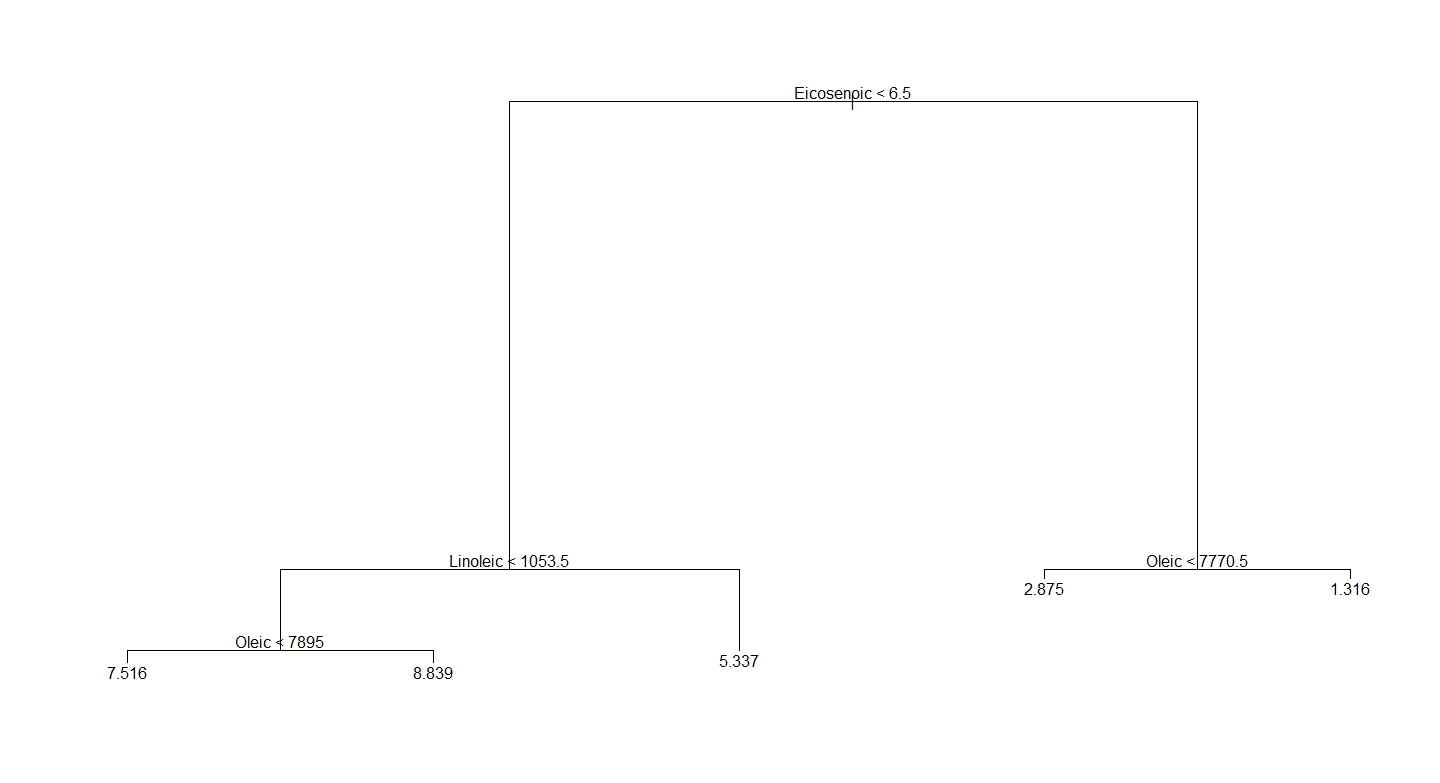
\includegraphics[width=0.95\linewidth]{./DAquiz6q4a}
\caption{}
\label{fig:DAquiz6q4a}
\end{figure}
\subsection*{Answer}
2.875. It is strange because Region should be a qualitative variable - but tree is reporting the average value of Region as a numeric variable in the leaf predicted for newdata.

\newpage
%-------------------------------------------------------%
\subsection*{Question 5}
Suppose that I fit and prune a tree to get the following diagram. What area
would I predict for a new value of:
\begin{framed}
\begin{verbatim}
olive.tree <- tree(as.factor(Area) ~ Palmitic + 
         Palmitoleic + Stearic + Oleic + Linoleic + 
         Linolenic + Arachidic + Eicosenoic, data=olive)

plot(olive.tree); text(olive.tree)
\end{verbatim}
\end{framed}
\begin{figure}[h!]
\centering
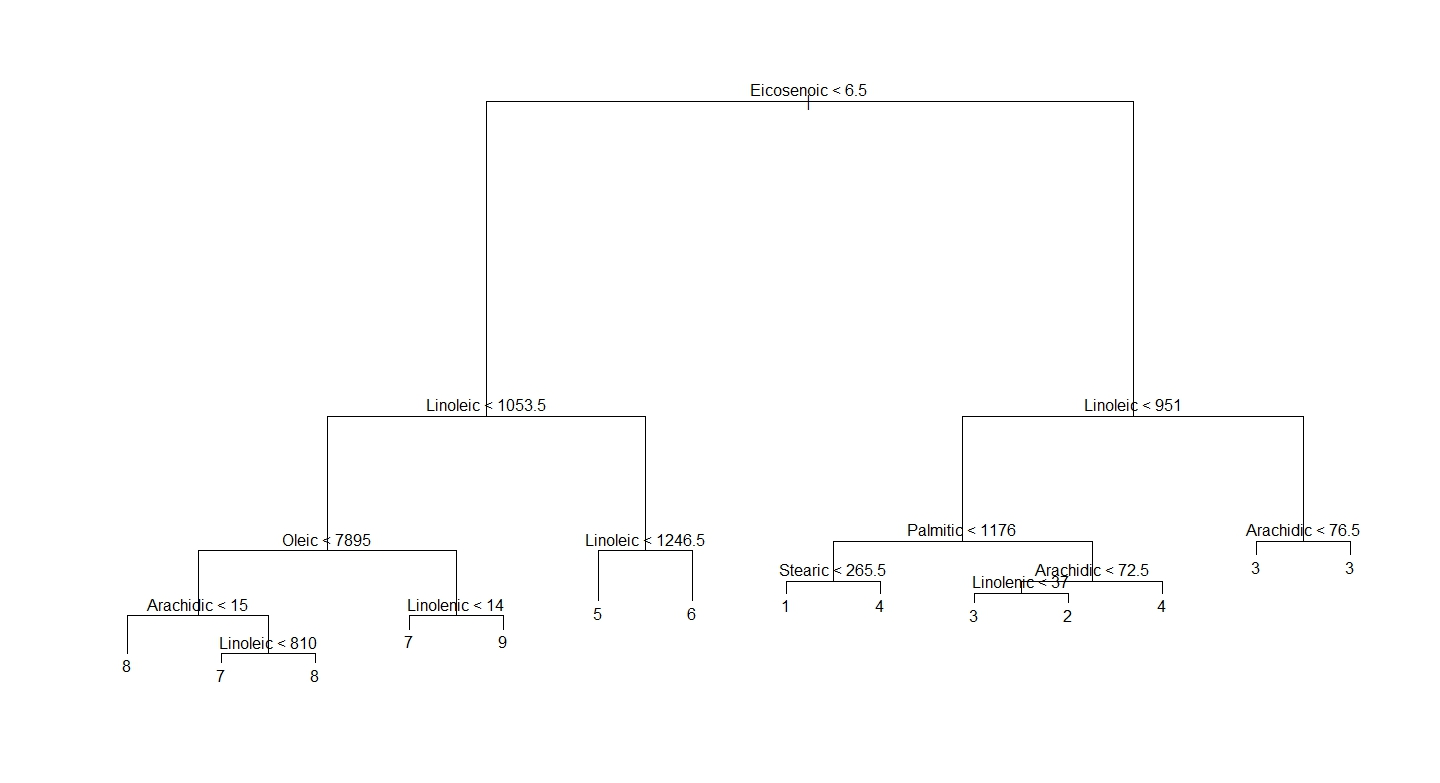
\includegraphics[width=1.19\linewidth]{./DAquiz6q5a}
\caption{}
\label{fig:DAquiz6q5a}
\end{figure}
The \texttt{prune.tree()} command determines a nested sequence of subtrees of the supplied tree by recursively “snipping” off the least important splits in the regression tree.
\begin{framed}
\begin{verbatim}
olive.pruned <- prune.tree(olive.tree,best=6)

plot(olive.pruned); text(olive.pruned)
\end{verbatim}
\end{framed}
\begin{figure}[h!]
\centering
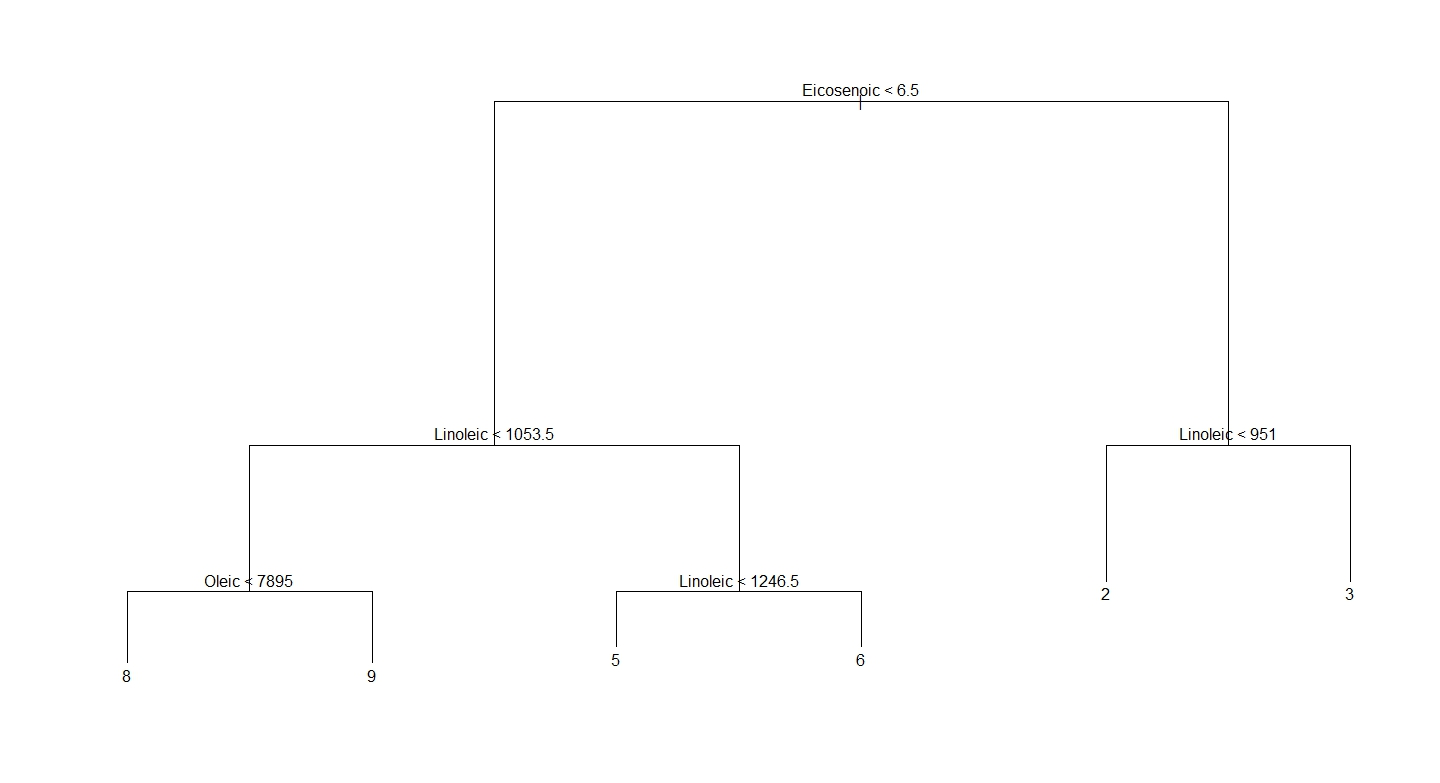
\includegraphics[width=1.19\linewidth]{./DAquiz6q5b}
\caption{}
\label{fig:DAquiz6q5b}
\end{figure}
\newpage
\begin{framed}
\begin{verbatim}
newData = data.frame(Palmitic = 1200, Palmitoleic = 120, 
          Stearic=200, Oleic=7000, Linoleic = 900, 
          Linolenic = 32, Arachidic=60, Eicosenoic=6)

predict(olive.pruned, newData)
\end{verbatim}
\end{framed}

\begin{verbatim}
predict(olive.pruned, newData)
  1 2 3 4 5 6         7         8 9
1 0 0 0 0 0 0 0.4842105 0.5157895 0
\end{verbatim}
\end{document}
